\documentclass[11pt,a4paper]{article}
\usepackage[margin=25mm,top=22mm,bottom=23mm]{geometry}
\usepackage{amsmath,amssymb,amsthm,booktabs,tikz,xcolor}
\definecolor{ink}{RGB}{19,84,82}
\definecolor{faint}{RGB}{242,248,246}
\usepackage[colorlinks=true,linkcolor=ink,urlcolor=ink,citecolor=ink]{hyperref}
\hypersetup{pdftitle={Minimum intersections at distances five and six on the double torus},
pdfsubject={A computer-assisted determination in the genus-two curve graph}}
\newtheorem{theorem}{Theorem}
\newtheorem{lemma}[theorem]{Lemma}
\newcommand{\C}{\mathcal C}
\newcommand{\code}[1]{\texttt{\detokenize{#1}}}
\newcommand{\repo}{https://github.com/LiquidGunay/short-twists-curve-graph}
\setlength{\parskip}{3pt plus .5pt}
\setlength{\parindent}{1.1em}
\setlength{\emergencystretch}{1em}
\raggedbottom
\begin{document}
\begin{center}
{\LARGE\bfseries Minimum intersections at distances five and six\\[3pt]
on the double torus\par}
\vspace{8pt}
{\small Computational research manuscript \(\cdot\) 26 November 2026}
\end{center}
\begin{abstract}
In the curve graph of the closed orientable genus-two surface, the least geometric
intersection numbers at distances five and six are 40 and 132. The same minima
hold when each distance is a lower bound. We encode a filling pair by a weighted
triangulation of the surface cut along one endpoint and a cyclic boundary gluing.
To exclude smaller examples, a census constructs short paths, using only elementary
curves that cross each band at most once and lower bounds at previously completed
distances. Two distance-six minimizers have absolute algebraic intersections
96 and 48, so they belong to different homeomorphism orbits. We verify the exact
distances of the examples separately using efficient geodesics.
\end{abstract}

\section{Statement and previous bounds}
Let \(S\) be the closed, connected, orientable surface of genus two. The vertices
of \(\C(S)\) are isotopy classes of essential simple closed curves. Distinct
vertices are adjacent when they have disjoint representatives. Write \(d(a,b)\)
for graph distance and \(i(a,b)\) for the minimum number of transverse crossings
of representatives. Define
\[
 m_d=\min_{d(a,b)=d}i(a,b),\qquad L_d=\min_{d(a,b)\ge d}i(a,b).
\]
\begin{theorem}\label{th:main}
On \(S\), \(m_5=L_5=40\) and \(m_6=L_6=132\).
\end{theorem}

Glenn, Menasco, Morrell and Morse determined \(m_4=12\) \cite[Thm.~1.6]{GMMM}.
For \(d\ge4\), the intersection growth inequality of Jin and Menasco gives
\(i(a,b)\ge12\,2^{d-4}\) on \(S\) \cite[Thm.~1.3]{JM}. It gives 24 and 48 at
distances five and six. Mahanta exhibited a specific distance-five pair with
144 crossings, obtained by one Dehn twist of a distance-four pair \cite[\S6]{M}.
A companion manuscript gives a distance-six example with 196 crossings and shows
that 196 is optimal among images of a distance-four pair under a single twist
\cite[\S7]{ST}. Theorem~\ref{th:main} allows all pairs, including those with a
separating endpoint. The earlier constructions answer a question about prescribed
twists that a minimum over all pairs cannot answer.

There are two numerical assertions behind the theorem. For every pair with at
most 131 crossings we exhibit, directly or by induction, a path of at most five
moves. We then specify one 132-crossing pair and exclude every path of at most
five moves for that particular pair. Its six-edge path supplies the opposite
distance bound. The two computations use different search criteria.

\clearpage
\section{Coordinates covering all filling pairs}\label{sec:atlas}
Put \(a,b\) in minimal position with \(N=i(a,b)>0\). At distance at least three
they fill \(S\), meaning that every complementary component is a disk. Cut along
\(a\). The resulting surface is either \(S_{1,2}\), or two copies of \(S_{1,1}\),
where the second index counts boundary components. The pieces of \(b\) form
\(N\) properly embedded essential arcs. Record parallel arcs by one band and
its width. Upon collapsing the two boundary circles to ideal vertices, a disk with
\(2k\) alternating sides becomes an ideal \(k\)-gon. Remove the bigons between
parallel arcs, and triangulate each remaining polygon by diagonals of width zero.
The cut surface has Euler characteristic \(-2\). The equations \(3F=2E\) and
\(F-E=-2\) give four ideal triangles and six edges across its components.

Number the sides of four oriented triangles \(0,\ldots,11\) and put
\(\rho=(0\,1\,2)(3\,4\,5)(6\,7\,8)(9\,10\,11)\). A fixed-point-free
involution \(\tau\) glues sides in pairs with opposite orientations. The cycles
of \(\rho\tau\) are the boundary circles. Of the \(11!!=10{,}395\) involutions,
4,563 have two cycles. They form six orbits under the \(4!\,3^4=1{,}944\)
permutations of triangles and rotations of their sides. To verify these counts
we enumerate every involution, generate the orbit of each listed representative,
and test that these orbits are disjoint and their union is the full eligible set.
Both the Python and Lean implementations include this finite test.

\begin{lemma}\label{lem:cover}
Every ordered filling pair on \(S\) with \(N\) crossings occurs in at least one of
the six charts, for a nonnegative six-tuple \(w\) with \(\sum w_j=N\) and a
shift \(s\in\{0,\ldots,N-1\}\).
\end{lemma}
\begin{proof}
Use the triangulation constructed above, with width zero on every added edge.
Each boundary circle meets precisely \(N\) arc ends, one for each crossing of
\(a\). The cyclic order of the ends is determined by the order of the sides and
the reversed order of parallel strands at the other end of a band. After
reversing the order on the second circle, any orientation-compatible boundary
identification sends position \(j\) to \(j+s\bmod N\). Changing the collar by
a full twist changes the marking by a homeomorphism fixing \(a\), which
preserves distance and intersection. The original \(b\) traverses all \(N\)
arcs as a single circle. The test for one component retains it.
\end{proof}

There is an elementary check on the width enumeration. If \(q_j\) counts the
ends of edge \(j\) at the first ideal vertex, then \(q_j\in\{0,1,2\}\).
Balance is equivalent to \(\sum_j(q_j-1)w_j=0\) together with \(\sum_jw_j=N\).
In each of the six charts two edges have distinct \(q_j\). Choose four
nonnegative widths freely up to their remaining total and solve both linear
equations for the other two. Retaining their nonnegative integral solutions
exhausts precisely the balanced six-tuples.

\begin{center}
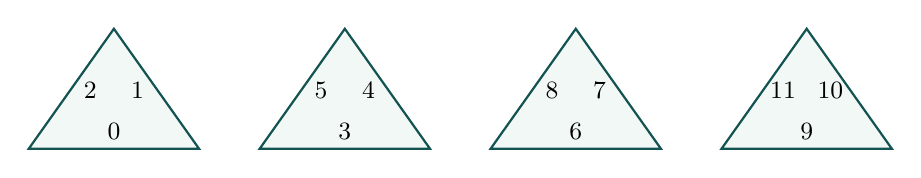
\begin{tikzpicture}[scale=.94, every node/.style={font=\small}]
\foreach \x/\base/\rightedge/\leftedge in {0/0/1/2,3.12/3/4/5,6.24/6/7/8,9.36/9/10/11}{
  \begin{scope}[xshift=\x cm]
    \draw[fill=faint,draw=ink,thick] (0,0)--(2.3,0)--(1.15,1.62)--cycle;
    \node at (1.15,.23) {\base};
    \node at (1.47,.78) {\rightedge};
    \node at (.83,.78) {\leftedge};
  \end{scope}}
\end{tikzpicture}

{\small The chart for the extremal examples pairs sides
\((0,3),(1,4),(2,6),(5,9),(7,10),(8,11)\).
The six widths in Table~\ref{tab:examples} follow this order.}
\end{center}

\clearpage
\section{A lower bound by exhibiting short paths}
For a threshold \(t\le L_k\), a curve \(z\) disjoint from \(a\), or isotopic to
it, gives the implication
\[
              i(z,b)<t \quad\Longrightarrow\quad d(a,b)\le k.
              \tag{1}\label{eq:sieve}
\]
Indeed \(d(z,b)<k\) and \(d(a,z)\le1\). This makes a search for cheap
neighbors sufficient to eliminate an input. The remaining inputs are kept
whenever the search fails.

For the first cut, take a circuit in the dual graph of the four triangles
that crosses each edge at most once. Within every triangle join the selected
sides by disjoint chords. A nonempty connected circuit gives an embedded
curve. Its dual edge path is cyclically reduced and nontrivial in the spine
of the cut surface. Cutting along an essential circle gives
\(\pi_1\)-injective components, so the curve is essential in \(S\) as well.
Its crossings with \(b\) are bounded by the sum of the widths of the edges
it crosses. This test is valid for every boundary shift at once.

For width vectors that survive, glue the boundaries and trace \(b\). Discard
gluings giving several components. Given the signed order of the crossings
of a connected pair \(x,y\), walk the sides of its regular neighborhood.
For \(N>0\) and \(f\) boundary cycles, its genus \(h\) satisfies
\(2-2h-f=-N\). If the complementary components have genera \(g_j\) and
boundary counts \(b_j\), Euler characteristic gives
\(2=h+\sum_j(g_j+b_j-1)\). Thus \(h=2\) exactly when every component is a
disk. Otherwise an essential boundary of the neighborhood gives a common
disjoint vertex. If every boundary were inessential, its disk would lie
outside the connected neighborhood containing the essential curves, and the
complement would consist of disks. A zero-crossing pair already has distance
at most one.

For a filling pair, collapse its rectangular bands again. Enumerate subsets of
the bands, pair the selected sides by noncrossing chords inside each complementary
polygon, and trace the resulting circuits. Keep connected curves only. Each
chosen band is crossed once. Record the resulting intersections in order
along the circuit and sort them along the original \(y\) to obtain the
child diagram \((z,y)\). These representatives are in minimal position.
A bigon disjoint from \(x\) would give a return across a properly embedded
arc already crossed at most once. If a bigon met \(x\), an outermost component
of \(x\) inside it would instead give a bigon for \(x,y\). The same argument
in the triangulated version uses normality to exclude a return across an
edge lift. At each step we can apply~\eqref{eq:sieve}, detect a common neighbor,
or recurse with the remaining distance budget reduced by one. A positive return
therefore certifies a path of at most the stated length.

The induction starts with \(L_3\ge4\). For \(N=1,2\), the required number
\(N-2\) of ribbon boundary cycles is impossible. For \(N=3\), fix crossing
1 as the initial label of the second curve. Each of the two orders of the
other labels and all eight sign choices give three boundary cycles. Filling
would require one. The census then proves successively \(L_4\ge12\),
\(L_5\ge40\) and \(L_6\ge132\).

\clearpage
\section{The finite calculation}
For a given target \(d\), the direct verifier uses only thresholds from
strictly lower distances. It tries every balanced width vector, including
zero widths, and all \(N\) shifts for each vector surviving (1). It tries the
short-path test in both endpoint orders as needed. Table~\ref{tab:census}
counts chart presentations, so multiple presentations of the same pair
contribute separately.

\begin{table}[h]\centering
\begin{tabular}{@{}crrrr@{}}\toprule
Target \(d\)&\(N\) searched&Width vectors after (1)&Gluings&Connected\\\midrule
4&1--11&151&1,598&360\\
5&1--39&62,249&2,271,417&566,002\\
6&1--131&17,383,334&2,123,473,921&540,360,860\\\bottomrule
\end{tabular}
\caption{Every connected diagram in each row has a path of at most \(d-1\) moves.
No diagram remained unresolved.}\label{tab:census}
\end{table}

A separate discovery implementation fan-triangulates the polygons and keeps
one width vector per chart symmetry orbit. It uses different endpoint labels
and generates balanced widths by partitioning edges according to their boundary
incidences. On \(48\le N\le131\) it retained the same 17,383,334 width vectors
before symmetry reduction and 4,237,317 after it. It traced 517,692,279 gluings
and obtained 132,061,336 connected presentations. All were excluded by
short-path witnesses or previously established thresholds. The direct run in
Table~\ref{tab:census} uses no width-vector symmetry reduction.

The extremal pairs below use the chart shown in Section~\ref{sec:atlas}. Begin each
cycle of \(\rho\tau\) with its least side. The first boundary runs through
\((0,4,2,7,11,6)\) and the second through \((1,5,10,8,9,3)\). Expand each side
to its width. Number the two ends of the \(j\)-th strand in an edge consecutively
as \(2j,2j+1\), with \(j\) starting at zero and increasing across bands.
At the lesser side of each paired edge list its even ends in increasing order,
and at its mate list its odd ends in decreasing order. Reverse the entire second
boundary list, then identify its position \(j+s\) with position \(j\) of
the first list, modulo \(N\). The seam is \(a\). Following arcs across it gives \(b\).

\begin{table}[h]\centering
\begin{tabular}{@{}crcrrr@{}}\toprule
\(d(a,b)\)& Six widths & Shift \(s\) & Squares & Hexagons & \(|[a]\cdot[b]|\)\\\midrule
5 & \((2,11,7,7,2,11)\)&4&34&4&0\\
6 & \((30,30,6,6,30,30)\)&13&126&4&96\\
6 & \((29,30,7,7,30,29)\)&13&126&4&48\\\bottomrule
\end{tabular}
\caption{Explicit pairs attaining the minima. Their width sums are 40, 132, and 132.}\label{tab:examples}
\end{table}

The boundary identifications yield a single \(b\) in each case. The face
profiles in Table~\ref{tab:examples} have \(N-2\) faces, all disks in the
capped ribbon surface. Thus the surface has genus two and contains no
complementary bigon. By the bigon criterion these crossing counts are geometric.
Summing the crossing signs gives the algebraic intersection. Its absolute
value survives endpoint exchange, curve orientation changes and surface
homeomorphisms of either orientation. The last two rows therefore represent
inequivalent unordered pairs.

\clearpage
\section{Verifying the two distances}
For a proposed budget \(B\ge3\), triangulate the complement after cutting
along \(a\), as above. If the true distance is \(\ell\) with \(3\le\ell\le B\),
the efficient-geodesic theorem supplies a shortest path whose first neighbor
meets each of the six reference arcs at most \(\ell-1\) times
\cite[Thm.~1.1 and pp.~3--4]{BMM}. Enumerate six weights in
\(\{0,\ldots,B-1\}\). In a triangle with edge weights \(u,v,w\), the number
of strands joining the first two edges is \((u+v-w)/2\). Apply this formula
cyclically and retain nonnegative integers. Gluing the triangle patterns and
retaining single circles gives all required first moves. Trace the child pair
and recurse with budget \(B-1\). At budget two apply the ribbon genus test.
Peripheral curves on the cut surface give a repeated vertex on \(S\), which
can be removed. An efficient first move exists at each filling stage of a
shortest path, so a negative result now excludes every shortcut.

The optimized test also uses the original-edge bound from
\cite[Prop.~3.7]{BMM} when all six edges come from the second curve. On the
first 132-crossing pair, testing budget five in this version visits 1, 80, 2,336
and 14,160 diagrams at budgets five, four, three and two. Every terminal
diagram fills \(S\). A separate run uses the larger uniform bound \(B-1\)
at every stage and visits 1, 192, 14,712 and 429,456 diagrams at the same
budgets. Both versions exclude the shorter paths for all three witnesses.
One successful path for the first 132-crossing example starts with four moves
whose successive normal coordinates, in the program's local edge order, are
\[
 (0,0,0,1,1,0),\quad(0,0,0,1,0,1),\quad
 (1,1,0,0,0,0),\quad(0,1,1,1,0,0).
\]
The remaining pair crosses five times and its regular neighborhood has genus
one, so it admits a two-edge path. The analogous three initial moves for the
40-crossing example leave a genus-one neighborhood with three crossings.
Together with Table~\ref{tab:census}, this proves Theorem~\ref{th:main}.

\paragraph{Reproducibility.}
The \href{\repo/tree/main/computations/minimum}{computational supplement}
includes both census programs, row-level counts, the three signed crossing words,
and the endpoint verifier. The \href{\repo/blob/main/proof/MinimumExamples.lean}{Lean
file} reconstructs the examples and checks their face profiles and distance
decisions. Its surface-distance theorems take an explicit geometric
interpretation of the checker as a hypothesis. The global census and its
topological coverage are justified by the programs and the arguments above.

\begin{thebibliography}{9}\small
\bibitem{BMM} J. Birman, D. Margalit and W. Menasco. Efficient geodesics and an effective
algorithm for distance in the complex of curves. \emph{Math. Ann.} \textbf{366}
(2016), 1253--1279. \href{https://arxiv.org/abs/1408.4133}{arXiv:1408.4133}.
\bibitem{GMMM} P. Glenn, W. Menasco, K. Morrell and M. Morse. MICC: A tool for computing
short distances in the curve complex. \emph{J. Symbolic Comput.} \textbf{78}
(2017), 115--132. \href{https://arxiv.org/abs/1408.4134}{arXiv:1408.4134}.
\bibitem{JM} X. Jin and W. Menasco. Super efficient geodesics in the complex of curves.
\href{https://arxiv.org/pdf/2008.09665v4}{arXiv:2008.09665v4}, Thm.~1.3.
\bibitem{M} K. Mahanta. Distance 5 curves in the curve graph of closed surfaces.
\href{https://arxiv.org/pdf/2211.15290v3}{arXiv:2211.15290v3}, \S6.
\bibitem{ST} \emph{Short Dehn twists at distances five and six on the closed genus-two
surface}. \href{\repo/blob/main/paper/short-twists.pdf}{Companion manuscript}, 2026.
\end{thebibliography}
\end{document}
